\documentclass[11pt,a4paper,twoside]{article}
\usepackage{a4wide}	% für gut definierte Seitenränder und Platzausnutzung
\usepackage[utf8x]{inputenc}	% für Umlaute
\usepackage{amssymb,amsmath}
\usepackage[pdftex]{graphicx}
\usepackage{epstopdf}
\usepackage{siunitx}	% für SI-Einheiten; siehe http://mirror.unicorncloud.org/CTAN/macros/latex/contrib/siunitx/siunitx.pdf
\usepackage{listings} 	% für Einbinden von Quellcode
\usepackage{color}	% für das Einfärben von eingebundenem Quellcode
\usepackage{longtable}	% für das Erstellen mehrseitiger Tabellen
\usepackage[german]{isodate} % Datumformatierung für \today
\usepackage{marvosym}

% declaring custom units
\DeclareSIUnit \mag {mag}
\DeclareSIUnit \parsec {pc}
\DeclareSIUnit \AU {AU}

% format angle display
\sisetup{add-arc-degree-zero}
\sisetup{add-arc-minute-zero}
\sisetup{add-arc-second-zero}
\sisetup{arc-separator = \,}


%Befehl, um Quellcode einzufügen: 
%\lstinputlisting[caption = {``title``}, captionpos = b, language=C++]{data.cpp}

%Befehl, um Graphik einzufügen:   
%\begin{figure}
%  \centering
%  \includegraphics[width=0.7\textwidth, angle=-90]{center_diff.eps}
%  \caption{centered differencing at t = 4}
%\end{figure}

% Befehl für kein ``\noindent mehr''
\setlength\parindent{0pt}

%\lstset{numbers=left}

\newcommand{\op}[1]{\operatorname{#1}}

\lstset{
   basicstyle=\scriptsize\ttfamily,			% grundlegendes Design
   keywordstyle=\ttfamily,				% Design von Schlüsselwörtern (Codebefehle wie Variablentypen, Schleifenbefehle u.Ä.)
   stringstyle=\ttfamily,				% Design von Variablen
   commentstyle=\ttfamily\color{blue},			% Design von Kommentaren
   showstringspaces=false,				% Leerzeichen in Strings darstellen?
   flexiblecolumns=false,				% dynamische Spaltenbreite?
   tabsize=2,						% Länge des Tabulators
   % Einstellung der Zeilennummerierung:
   numbers=left,					% Position der Nummern
   numberstyle=\tiny,					% Größe der Nummern
   numberblanklines=true,				% Leerzeilen durchnummerieren?
   numbersep=20pt,					% Platz zwischen Nummern und Code
   xleftmargin=30pt					% Platz zum linken Seitenrand
 }
 
%opening
\title{\LARGE \underline {Sheet 2}}
\author{Johannes Haux \\ Florian Trost \\ Elsa Wilken}
\date{\today}


\begin{document}

\maketitle
\thispagestyle{empty}

\begin{center}
  Astronomical Techniques (MKEP5) \\
  \baselineskip35pt
  by Prof. Dr. Stefan Wagner and Priv.-Doz. Dr. Thorsten Lisker \\
  \baselineskip60pt
  Ruprecht Karl University of Heidelberg
\vskip 40pt
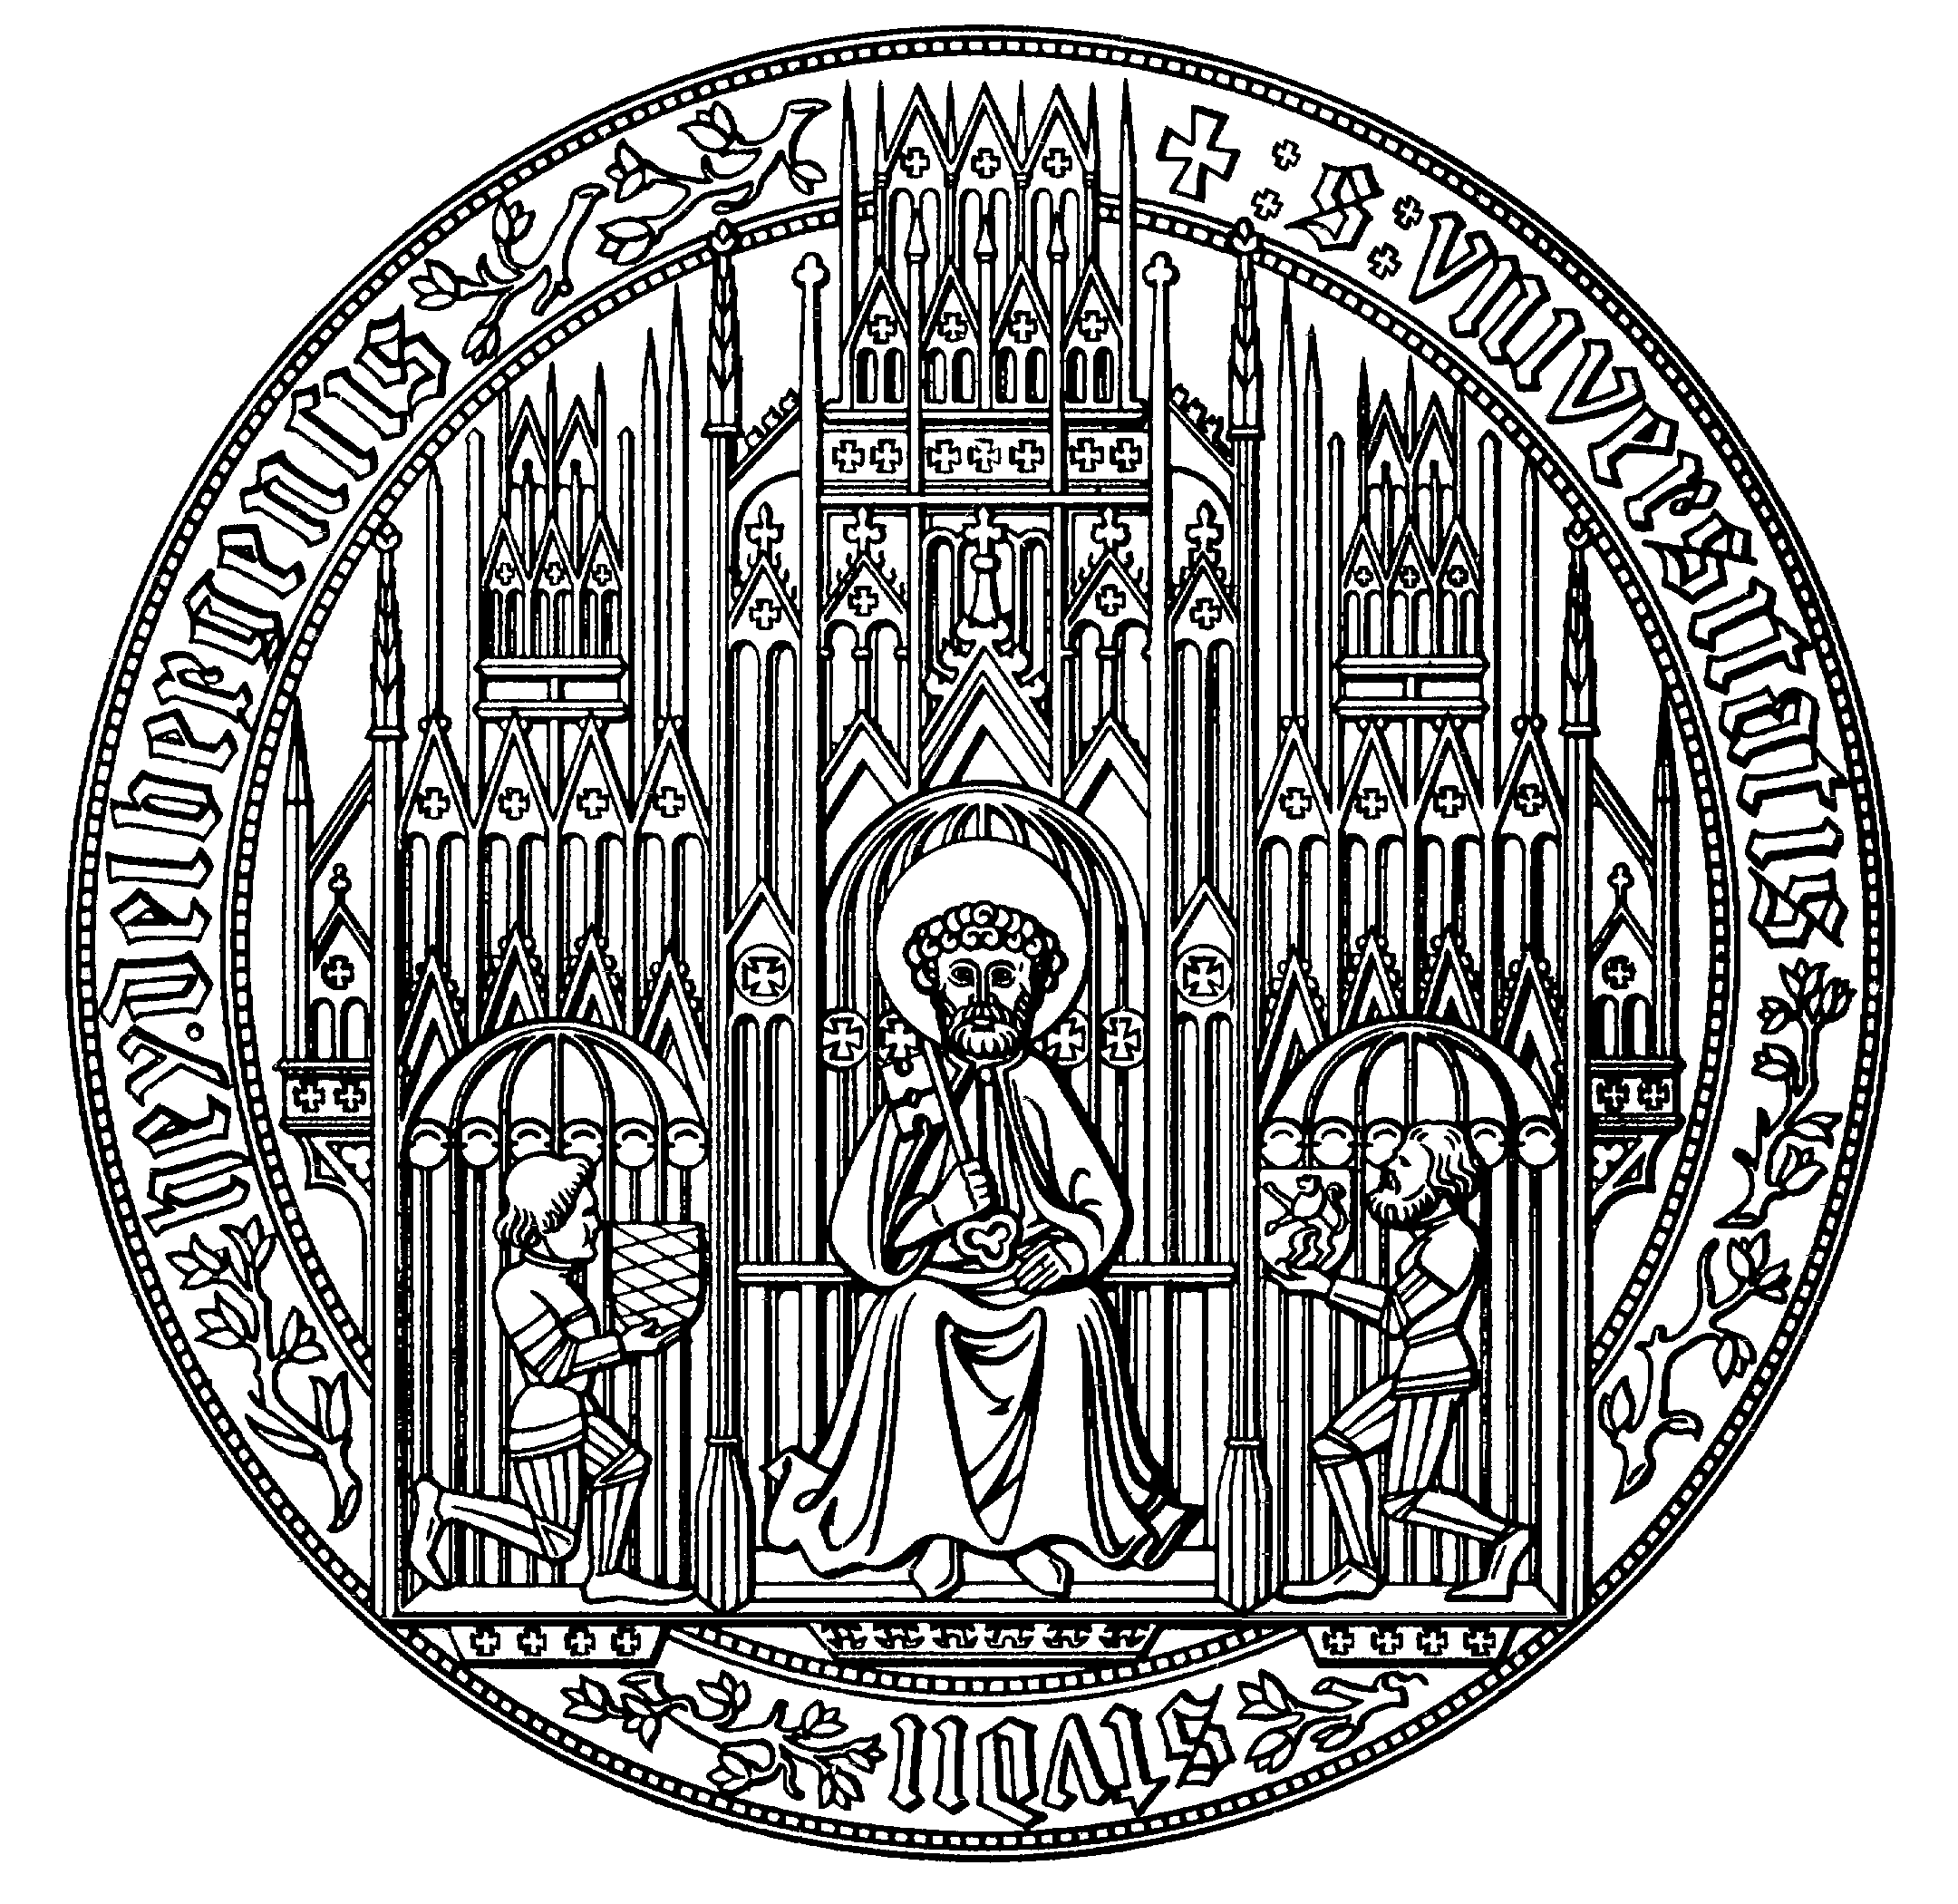
\includegraphics[width=5cm]{pic/UniHD.png}

\end{center}

\newpage
\setcounter{page}{1}		% set page count to start with 1 here

\section*{Exercise A.} 

\section*{Exercise B.}
The North America Nebula and the Pelican Nebula shown on the sheet are
ionized by a massive, main-sequence star of spectral type O5V, located at 
$RA = \SI{20}{^\hour}\SI{55}{^\minute}\SI{51.3}{^\second}$ $DEC = \ang{43;52;25}$.
We want to observe it using the \SI{2.1}{\meter} telescope of the San Pedro 
Martir Observatory (at \ang{31.0442} North, in Mexico). This star has, outside 
the Earth atmosphere, a colour $(U – V) = \SI{-1.42}{\mag}$ and an absolute 
magnitude $M_V = \SI{-5.21}{\mag}$ (at a distance of \SI{610}{\parsec}). Compute
the observed colour at three different hour angles $HA = \SI{-4}{\hour}; 
\SI{0}{\hour}; \SI{+3}{\hour}$, knowing that the atmosphere extinction 
coefficients are $k_U = \SI{0.53}{\mag\per airmass}$ and 
$k_V = \SI{0.18}{\mag\per airmass}$.
Briefly comment your results. (8 points)
\newline

The apparent magnitude and thus also the color of the observed star depend on
the amount of atmosphere, that the light has to pass before hitting the 
CCD or the eye. This amount $X$ can be calcualated in units airmass via the 
zenith distance $z$:
\begin{align}
    X &= \frac{\SI{1}{airmass}}{\cos(z)} \;.
\end{align}
As $z = \ang{90} - h$ we find that $\cos(z) = \cos(\ang{90} - h) = \sin(h)$,
which is given via the hour angle $HA$, the latitude of the observer $\Phi$
and the declination $DEC$ of the star:
\begin{align}
    \cos(z) = \sin(h) &= \cos(\Phi)\cos(DEC)\cos(HA) + \sin(\Phi)\sin(DEC) \;.
\end{align}
This dependence is visualized in figure \ref{fig:X} in the lower plot.

Now we can calculate the apparent magnitude $m$, using the extraatmospheric
magnitude $m_0$ and the atmosphere extinction coefficient $k$:
\begin{align}
    m &= m_0 \cdot kX ;.
\end{align}
Knowing dependence of the apparent and absolute magnitude $m_{0,V}$ and $M_V$ 
on the distance $d$ as well as the extraatmospheric color $(U-V)_0$ we can 
calculate the extraatmospheric magnitude $m_{0,U}$ in the $U$-band and the
observed color:
\begin{align}
    m_{0,V} &= 5\log_{10}(d) - 5 + M_V \;,\\
    m_{0,U} &= (U-V)_0 + m_{0,V} \;,\\
    (U-V)_{obs} &= m_{0,U} \cdot k_U X - m_{0,V} \cdot k_V X \;.
\end{align}
The dependence of color on the hour angle is again visualized in the upper plot
in figure \ref{fig:X}. The results or the three given angels are given in table
\ref{tab:col}.
\begin{table}
\centering
\begin{tabular}{c|c}
$HA$    & $(U-V)_{obs}$ \\
-4      & \num{0.822672456176}  \\
0       & \num{0.562563507003}  \\
3       & \num{0.690441039578}  \\
\end{tabular}
\caption{Results for exercise B.}
\label{tab:col}
\end{table}

\begin{figure}
\centering
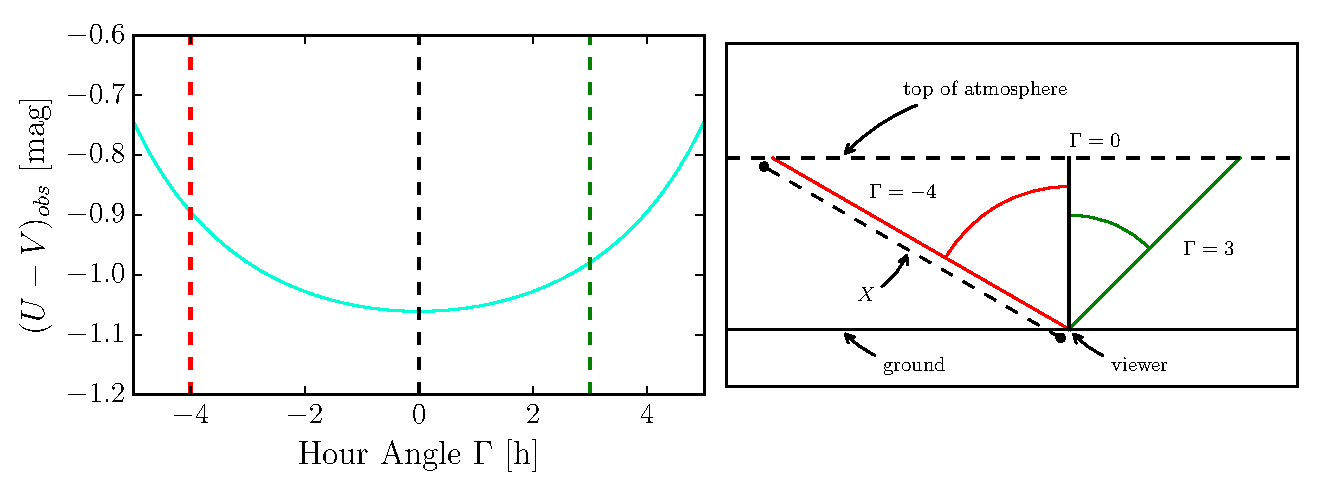
\includegraphics[width=10cm]{pic/umv}
\caption{$\land$: Dependence of color on the hour angle. $\lor$: The dependence
         of X on the hour angle. At $HA = 0$ we observe 1 airmass.}
\label{fig:X}
\end{figure}


\section*{Exercise C.} 
We observed the Galactic open cluster shown in Fig. 3 through the B and V
filters, and measured the B and V magnitudes for 21 of its member stars. These 
are listed in the attached file: \verb+BV_photometry.dat+. They have been 
already corrected for atmospheric extinction, and their associated errors can 
be neglected for the purpose of this exercise.

\begin{enumerate}
\item Construct their colour-magnitude diagram (CMD) V vs (B-V). (2 point)
\item In the same diagram plot the V magnitudes and (B-V) colours listed in the 
attached file: \verb+age_3.5gyr.dat+, knowing that the cluster is at a distance
of \SI{890}{\parsec}. The file \verb+age_3.5gyr.dat+ is the isochrone computed for 
the age of the cluster, estimated by previous studies to be 3.5 Gyr. (2 points)
\item Compare the locus of the isochrone in the CMD with the measured 
photometric points: what do you find? Is that what you expected? (2 points)
\end{enumerate}

In figure \ref{fig:cmd} one can find the plot of the data given for this 
exercise. 
The isochrone data have to be corrected as they are given in units of absolute
magnitude, while the other data is in units of apparent magnitude. For this
we use the relation between apparent Magnitude $m$ and absolute magnitude $M$
given the distance of the cluster $d = \SI{890}{\parsec}$,
\begin{align}
    m &= 5\op{log}_{10}(d) - 5 + M \;.
\end{align}

The locus of the isochrone is shifted into the red with respect to the CMD. 
This is probably due to the age of the cluster as with age the light of the 
stars shifts to the red.


\begin{figure}
\centering
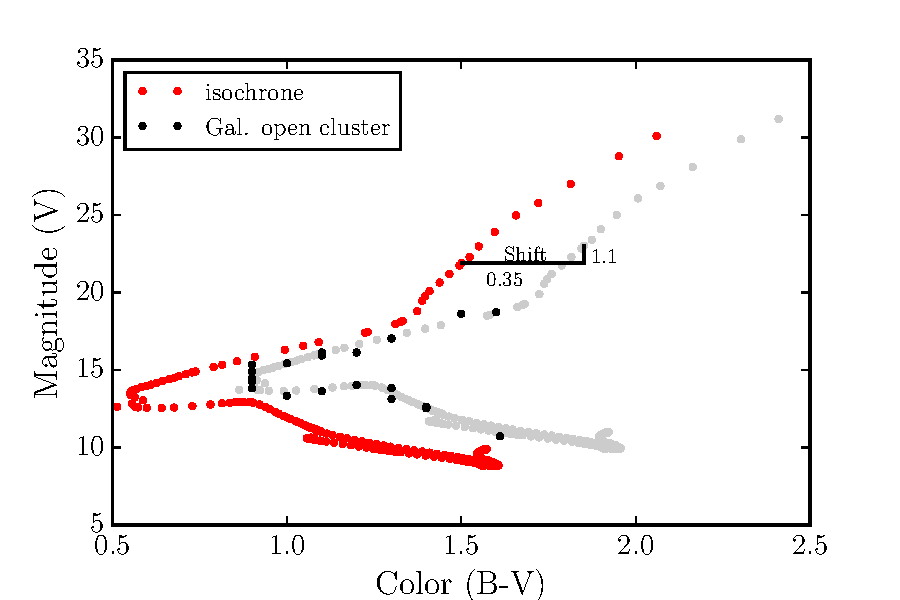
\includegraphics[width=10cm]{pic/CMD}
\caption{Color Magnitude diagram of the cluster given in Exercise C. 
         Visualized in black is the observed data, in red the 
         isochrone-corrected data and in gray a shifted version of the 
         isochrone data. One can see that the isochrone is shifted into the 
         red.}
\label{fig:cmd}
\end{figure}

\section*{Exercise D}
The James Webb Space Telescope (JWST, NASA) has an effective diameter
$D = \SI{6.57}{\meter}$ (see Fig. 4 on the sheet). It also has an effective 
focal ratio $F = 20$, and is equipped with an optical-to-NIR imager (NIRCam) 
whose pixel has a length of \SI{18}{\micro\meter}. What is the image pixel 
scale in arcseconds? (2 points)
\newline

We know that the pixelscale $q$ is given as the pixel length $l_{pix}$ divided 
by the focal length $f$, which is given as the focal ration $F$ times the 
diameter of the objective:
\begin{align}
    f &= FD \;, \\
    q_{rad} &= \frac{l_{pix}}{f} \;.
\end{align}
This gives the result in radians, this we have to multiply by the factor
$f_{radian \rightarrow arcsec}$:
\begin{align}
    f_{radian \rightarrow arcsec} &= 
    \underbrace{\frac{\ang{180}}{\pi}}_{radian \rightarrow degrees} \cdot 
    \underbrace{60 \cdot 60 \frac{\si{\arcsecond}}{\si{\degree}}}_{
                degrees \rightarrow arcseconds}
\end{align}

Thus we find that the pixel scale $q$ is
\begin{align}
    q &= f_{radian \rightarrow arcsec} \cdot q_{rad} \\
    &= \SI{0.28}{\arcsecond} \;.
\end{align}


\section*{Exercise E}
HD 114762b is the first exoplanet ever discovered (in 1989 and confirmed in
1991), predating the detection of the better known 1992 planet found around the 
pulsar PSR B1257+12. HD 114762b is the companion of the F9V star HD 114762 at 
a distance of \SI{40.6}{\parsec} in the constellation of Coma Berenices.
At apastron the planet is \SI{0.471}{\AU} away from the star ($d_a$, 
perpendicular to the line of sight), while at periastron the distance 
planet - star is $d_p = \SI{0.235}{\AU}$ (perpendicular to the  line of sight).
$$\SI{1}{\AU} = \SI{1.496d13}{\centi\meter}$$

\begin{enumerate}
\item What is the minimum diameter $D$ a telescope should have to resolve this 
planet at periastron and apastron at $\lambda = \SI{7000}{\angstrom}$? 
(5 points)
\item The instrument WFC3-UVIS onboard the Hubble Space Telescope has a pixel 
scale of \SI{0.04}{\arcsecond\per pixel}. How many pixels do $d_p$ and $d_a$ 
correspond to? (2 points)
\end{enumerate}


\end{document}
